% g_star_comparison.tex — Effective DOF g_* AVE 343/4 vs SM 106.75 (Vol 9 Ch.12)
% Pure TikZ bar comparison (no pgfplots): two bars scaled to value, with the -21 DOF deficit.
% Bar width 0.06 cm per DOF unit: 85.75 -> 5.145 cm; 106.75 -> 6.405 cm.
\begin{figure}[htbp]
\centering
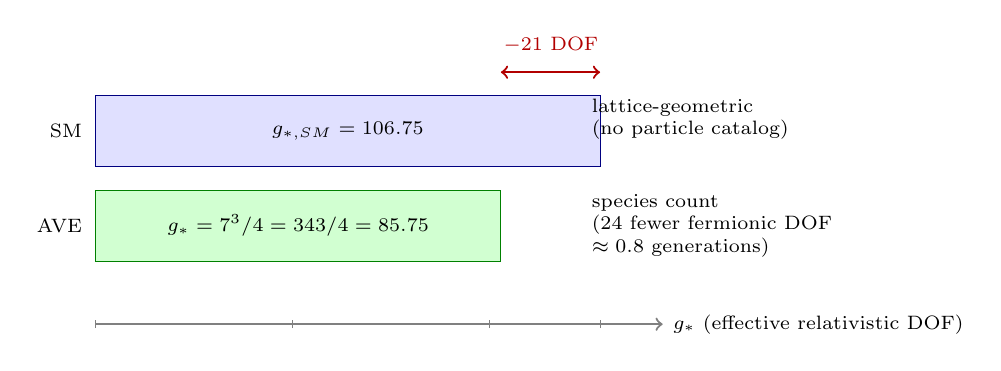
\begin{tikzpicture}[
    barlbl/.style={font=\scriptsize, align=left},
    val/.style={font=\scriptsize\bfseries}
]
    % axis baseline
    \draw[->, thick, gray] (0,-0.6) -- (7.2,-0.6) node[right, font=\scriptsize, black] {$g_*$ (effective relativistic DOF)};
    \foreach \x/\t in {0/0, 2.5/41.7, 5/83.3, 6.405/106.75} {
        \draw[gray] (\x,-0.65) -- (\x,-0.55);
    }

    % AVE bar: 85.75 * 0.06 = 5.145
    \fill[green!18, draw=green!50!black] (0,0.2) rectangle (5.145,1.1);
    \node[barlbl] at (-0.05,0.65) [left] {AVE};
    \node[val] at (2.57,0.65) {$g_* = 7^3/4 = 343/4 = 85.75$};

    % SM bar: 106.75 * 0.06 = 6.405
    \fill[blue!12, draw=blue!50!black] (0,1.4) rectangle (6.405,2.3);
    \node[barlbl] at (-0.05,1.85) [left] {SM};
    \node[val] at (3.2,1.85) {$g_{*,SM} = 106.75$};

    % deficit bracket
    \draw[<->, thick, red!70!black] (5.145,2.6) -- (6.405,2.6);
    \node[barlbl, text=red!70!black] at (5.78,2.95) {$-21$ DOF};
    \node[barlbl] at (8.0,2.0) [text width=3.4cm] {lattice-geometric\\(no particle catalog)};
    \node[barlbl] at (8.0,0.65) [text width=3.4cm] {species count\\(24 fewer fermionic DOF\\$\approx 0.8$ generations)};
\end{tikzpicture}
\caption{Effective relativistic degrees of freedom: AVE lattice-geometric $g_* = 7^3/4 = 85.75$ (from $\nu_{vac} = 2/7$, no particle catalog) vs the Standard Model species count $g_{*,SM} = 106.75$ (Vol.~9 Ch.~12 \S\ref{sec:vol9_cosmo_dark_sector}). The $-21$ DOF deficit forward-predicts a primordial GW background $\sim 7.6\%$ stronger ($\Omega_{GW} \propto g_*^{-1/3}$) and the electroweak-epoch expansion rate $\sim 10.4\%$ slower. Canonical at \kbleaf{effective-dof-g-star.md} (\texttt{clm-uu6dl5}); divergence row C12-G-STAR.}
\label{fig:vol9_g_star_comparison}
\end{figure}
